\documentclass[fontsize=11pt, paper=a4, parskip=half]{scrartcl}
\pagestyle{plain}

\usepackage[T1]{fontenc}
\usepackage[utf8]{inputenc}
\usepackage[english]{babel}
\usepackage{url}
\usepackage{hyperref}
\usepackage{lipsum}
\usepackage{graphicx}
\usepackage[perpage]{footmisc}
\usepackage{tikz}

\newcommand{\foo}{\hspace{-2.3pt}$\bullet$ \hspace{5pt}}

\setkomafont{disposition}{\normalcolor\bfseries}

% In den folgenden Zeilen {...} jeweils durch die tatsächliche personen-/exposébezogene Angaben ergänzen
\title{
	HoneyHints \\ Extract non-trivial cowrie log information
}

\subtitle{Bachelor's thesis proposal}

\author{
	Dominic Rudigier
	\\
	\texttt{Dominic.Rudigier@student.uibk.ac.at}  
	\\ \\
	{11832156}
}

\begin{document}

\maketitle
\newpage
\section{Motivation}
% Lipsum durch tatsächlichen Exposé-Text ersetzen
Additional to our firewall and other security solutions a honeypot helps protect a network from hackers, designed to catch the hacker's attention. Vulnerable as an easy target it grants possibilities to track the hacker's activities. Once connected to the internet the honeypot generates log files for all events, but the gathered information is hard to handle. If the firewall fails to prevent attacks we know how far the hacker has invaded our network and whether there are dangers of accessing company data. \\
One might ask why there is a need for additional tools as the quantity of honeypots and related tools is already slightly overwhelming.\footnote{\url{https://github.com/paralax/awesome-honeypots}} \\
There are multiple tools available showing log files and statistics of honeypots but there are none to perform an intelligent and useful analyzation to extract non-trivial information to detect anomalies in the log data. These anomalies might be user/password combinations indicating new device vulnerabilities of specific vendors or similar. Furthermore, analyzing commands executed prior to disconnects of the honeypot might give us a chance to find ways to improve it as malware might have found some ways to detect honeypot systems executing common commands known to be honey. The goal of this work is to find new ways to batch process cowrie logs and extract useful information to provide a possibility to be one step ahead of the attacker and iteratively improve our deployed honeypots. 

\begin{figure}[ht!]
	\centering
	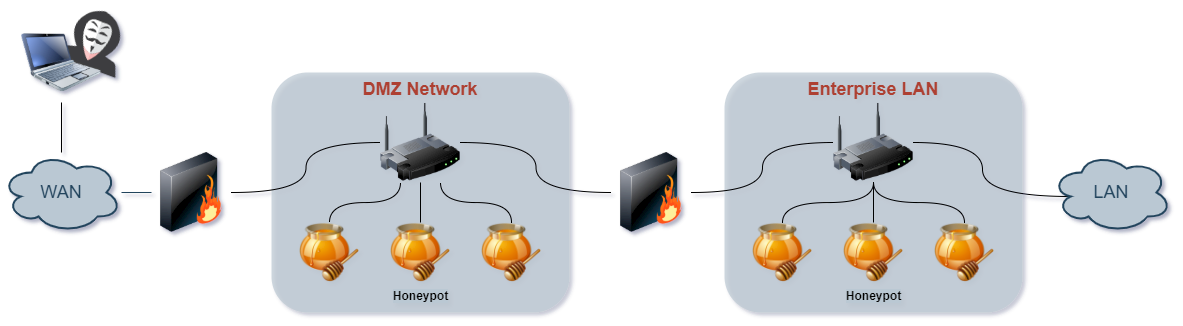
\includegraphics[width=\textwidth]{img/DMZ_Honeypot.png}
	\caption{Possible network infrastructure}
	\label{fig1}
\end{figure}

Imagine a scenario where an attacker has already access to our prevalent honeypots in a demilitarized zone and has connected to it. If our setup in this secured zone is similar to our enterprise network chances are high that we can spot common exploits or hopefully also zero-days if our honeypot is not detected. This possibility provides a huge advantage to secure our system from the maleficent actor and be one step ahead as we can further secure our enterprise LAN with all the knowledge gained. Therefore the main focus lies on techniques to adapt a honeypot to further hide it from the attacker to get quantitative information.

\pagebreak
\section{Status quo}
The current state of the art for logging brute-force attacks and shell interactions of connection-based intrusion attacks is a SSH and Telnet honeypot called Cowrie\footnote{\url{https://github.com/cowrie/cowrie}} by micheloosterhof (Github). Cowrie grants the possibility to catch attacker actions and provides logs  of all kinds like JSON, UML, TTY, Splunk HEC and different databases like MongoDB, SQLite and MySQL \cite{cowrie:artefacts}. Although there exist data analyzation platforms like Splunk Enterprise\footnote{\url{https://www.splunk.com/}} (which is not for free) with Cowrie analysis apps like Tango\footnote{\url{https://github.com/aplura/Tango}} they are all more concentrated on the individual analysis of honeypots and collection of statistics than on a severe analysis of individual attacker behaviors and action paths. Malware has become more intelligent recently which enlights the need for analysis and improvement of intrusion detection systems.\footnote{\url{https://www.avira.com/en/blog/new-mirai-variant-aisuru-detects-cowrie-opensource-honeypots}}

\section{Modus operandi}
\subsection{Goals}
The primary goal of the work is to batch process connection-based honeypot log data and extract useful information to improve existing systems and have a possibility to view interaction based attacker behavior. There are tons of attacks happening all the time, the tool should provide a possibility to detect anomalies in attacker behavior like sudden disconnects after specific commands or general log data anomalies not previously shown up. As an initial try the FReMP Stack\footnote{\url{https://fremp.github.io/}} is used to develop a web application to easily visualize python processed log files from a database. Research will show whether machine learning attempts could be helpful in detecting outliers for some cases or a manual analyzation is preferable, which is not clear yet. The software structure of the intended system can be viewed in \ref{fig2}. 
\begin{figure}[ht!]
	\centering
	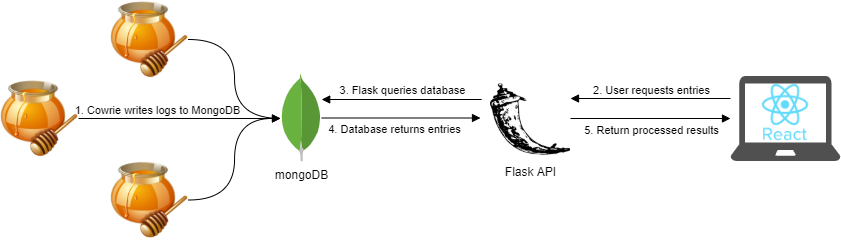
\includegraphics[width=0.8\textwidth]{img/FReMP.png}
	\caption{Web application infrastructure}
	\label{fig2}
\end{figure}

\subsection{Timeline}
\scalebox{1}{
	\begin{tabular}{r |@{\foo} l}
		February & Research ssh honeypots\\
		March & Set up multiple cowrie honeypots, test Splunk, test logging functionalities\\
		April & Start developing FReMP honeyview application (initially 2 honeypots)\\
		April & Research machine learning attempts of log anomaly detection\\
		April & Research batch-processing log data \& aggregating information \\
		April & Visualize pre-disconnect commands frequency\\
		May & Detect outliers for different log tables and display\\
		May / June & Extend functionality on n honeypots\\
		June & Handle bugs/improvements appeared during development process\\
		July & Dream: "Hints to improve honeypot x"\\
		July & Finish application\\
		August & Write thesis
	\end{tabular}
}

\subsection{Risks}
\begin{itemize}
	\item Gathering Data \\
	As the goal is to have test data for our web application in the first place there is a need to set up honeypots and create those log data for cowrie. With the attraction of attackers there is always a slight risk of them escaping our sandbox and using a honeypot as pivot node to penetrate productive systems. There were used dedicated droplets on DigitalOcean\footnote{ \url{https://www.digitalocean.com/}} to secure this. Props for the free credits.
	\item Database \\
	A database system with potential user connection data might attract some blackhats as well. A basic mongodb authentication and a firewall denying all incoming connections except for our honeypots and our webapp will grant proper security.
\end{itemize}

\pagebreak
\nocite{*}
\bibliography{literature}
\bibliographystyle{abbrv}
\end{document}
